% Adapted from the official ACM small-format Overleaf template, 28 September 2026.
% Classroom manuscript, not an accepted or published ACM article.
\documentclass[acmsmall,screen,nonacm]{acmart}
\usepackage{amsmath}
\usepackage{array,tabularx}
\newcolumntype{Y}{>{\raggedright\arraybackslash}X}
\usepackage{placeins}
\usepackage{xurl}
\acmJournal{CSUR}
\setcopyright{none}
\settopmatter{printacmref=false}
\begin{document}
\title[AI and Digital Twins for Smart Farming]{The Convergence of Artificial Intelligence and Digital Twins for Smart Farming: A Critical Review of Architectures, Applications, and Research Directions}
\author{Vineesh Cutting}
\affiliation{\institution{Indian Institute of Information Technology, Allahabad}\city{Prayagraj}\country{India}}
\renewcommand{\shortauthors}{Vineesh Cutting}
\begin{abstract}
Digital twins offer a way to connect agricultural observations, computational models, and management decisions, while artificial intelligence can support state estimation, forecasting, and optimisation within that connection. Their combination is particularly relevant to irrigation, where useful predictions must account for soil hydraulics, crop demand, uncertain weather, and actuator constraints. This critical narrative review examines agricultural digital-twin architectures and develops an irrigation-centred technical synthesis linking governing equations, model calibration, data assimilation, and physics-informed learning. Root-zone water balance and the Richardson-Richards equation provide the physical basis; crop models connect water availability to development and production; and physics-informed neural networks provide a possible route to inverse estimation and constrained approximation. The review distinguishes conceptual architectures, numerical demonstrations, and field implementations rather than treating them as equivalent evidence. A proposed closed-loop framework translates estimated soil moisture into constrained irrigation decisions and evaluates performance through moisture error, water-balance closure, metered irrigation volume, crop response, and operational reliability. An illustrative calculation demonstrates the conversion from root-zone depletion to irrigation depth and volume without claiming experimental validation. The central conclusion is that predictive accuracy alone is insufficient to establish agronomic value. Credible smart-farming digital twins require identifiable parameters, independent validation, explicit uncertainty, reliable physical feedback, and controlled comparisons of measurable outcomes. Research priorities include decision-aware calibration, multi-season validation, conservative hybrid models, and affordable deployment under intermittent connectivity.

\end{abstract}
\begin{CCSXML}
<ccs2012>
<concept><concept_id>10010147.10010341</concept_id><concept_desc>Computing methodologies~Modeling and simulation</concept_desc><concept_significance>500</concept_significance></concept>
<concept><concept_id>10010147.10010257</concept_id><concept_desc>Computing methodologies~Machine learning</concept_desc><concept_significance>300</concept_significance></concept>
</ccs2012>
\end{CCSXML}
\ccsdesc[500]{Computing methodologies~Modeling and simulation}
\ccsdesc[300]{Computing methodologies~Machine learning}
\keywords{Digital twin, artificial intelligence, smart farming, precision irrigation, soil moisture, model calibration, physics-informed neural networks, decision support}
\maketitle

\section{Introduction}

\label{sec:1}

Smart farming increasingly brings together observations of soil, crops, weather, and equipment. The scientific challenge is not simply to collect these observations, but to infer the condition of a changing biological system and decide what intervention is justified. A soil-moisture measurement, for example, is informative only in relation to its depth, calibration, crop rooting pattern, recent irrigation, and expected atmospheric demand. A prediction becomes operationally useful when it can change a decision while keeping the consequences of error visible.

Agricultural digital twins provide an organising framework for this relationship. Verdouw et al. \cite{R01} describe digital representations embedded in smart-farming management cycles. Pylianidis et al. \cite{R02} examine agricultural use cases and adoption pathways, while Purcell and Neubauer \cite{R03} review definitions, integration, and application maturity. A more recent review identifies continuing limitations in interoperability, cross-asset integration, and large-scale field validation \cite{R04}. Together these works motivate a distinction between an attractive digital representation and a functioning model-based management system.

Artificial intelligence (AI) can contribute several different capabilities: translating images into crop-state indicators, forecasting disturbances, approximating expensive simulators, detecting abnormal sensors, and learning components that are difficult to model explicitly. These functions should not be conflated. A model trained to reproduce historical irrigation actions may imitate an existing schedule without improving it. Likewise, a low soil-moisture prediction error does not establish that the same model can safely optimise future actions.

This review therefore asks three questions. What architecture connects an agricultural model to a physical decision loop? How can governing equations, calibration, and physics-informed learning support that architecture? What evidence is required to connect improved modelling to soil moisture, water consumption, and irrigation outcomes? Smart farming is considered broadly, but precision irrigation provides the detailed example because the chain from observation to action can be expressed quantitatively. The contribution is a critical synthesis and a proposed evaluation framework, not a new algorithm or a report of field experiments.


The specific contribution is an evidence-to-decision synthesis. Agricultural reviews explain integration and adoption \cite{R01,R02,R03,R04}; soil-water studies examine whether a model can recover states or fluxes \cite{R15,R16}; and irrigation-control work examines how predictions affect actions \cite{R18}. These contributions are complementary, but their validation targets are not interchangeable. This review connects them through four classification axes, a study-level comparison, and testable research gaps. It does not claim that its selected corpus exhausts the field or that a single model family is universally preferable.

Section~\ref{sec:2} states the evidence boundaries. Section~\ref{sec:3} develops the architecture and taxonomy; Sections~\ref{sec:4}, \ref{sec:5}, and~\ref{sec:6} connect governing physics, calibration, and learning. Section~\ref{sec:7} compares research approaches, and Section~\ref{sec:8} translates modelling into measurable decisions. Section~\ref{sec:9} sets out an evaluation agenda before the conclusions in Section~\ref{sec:10}.

\section{Review Approach and Evidence Boundaries}

\label{sec:2}

The research questions are introduced in Section~\ref{sec:1}.

This is a focused critical narrative review, not an exhaustive systematic review or meta-analysis. Targeted web searches and citation-led selection were used to locate agricultural digital-twin reviews, soil-water modelling foundations, physics-informed learning studies, and relevant irrigation and greenhouse applications. Searches combined terms including "digital twin smart farming", "agricultural digital twin irrigation", "Richards equation physics-informed neural network", and "model predictive control agro-hydrological systems". Publisher pages, author-hosted manuscripts, institutional repositories, FAO material, and an explicitly identified arXiv preprint were consulted. Bibliographic metadata were cross-checked against publisher or DOI records. The initial literature check was completed on 25 September 2026. Targeted source checks for the expanded comparison were performed on 28 September 2026; these did not constitute a new systematic search.

Sources were selected for their relevance to architecture, physical modelling, calibration, or measurable management outcomes. The resulting 20-reference set is purposive and English-language; it does not support estimates of publication prevalence or pooled effect sizes. Where only publisher summaries were accessible, interpretation is restricted to the reported scope and findings. One control study \cite{R18} is cited as a preprint and is not treated as peer-reviewed field evidence.

Three evidence levels are kept distinct: conceptual or review-level arguments; numerical or model-validation studies; and physical deployment studies. These levels address different questions. A numerical demonstration can validate an inverse modelling method but cannot establish seasonal water savings. A deployed platform can demonstrate integration while leaving the separate contribution of its AI component unresolved. Equations below summarise established formulations, whereas the proposed architecture, evaluation protocol, and worked example are the synthesis of this review.


\subsection{Extraction Criteria and Limits of Comparison}
\label{sec:extraction}
For the expanded comparison, each selected study is read against the same questions: what physical entity is represented; what observations or generated data are used; which model and learning method are involved; what outcome is evaluated; and what prevents the result from supporting a stronger claim? The detailed comparison in Section~\ref{sec:study-comparison} distinguishes full-text numerical evidence from publisher-accessible descriptions of deployment studies. An unavailable dataset identifier is recorded as unverified, not interpreted as proof that data do not exist.

The 20 sources serve different purposes: four agricultural architecture or review papers, one cross-domain classification, seven physical-modelling and estimation foundations, five physics-informed learning papers, and three application studies. These are roles within the selected corpus, not prevalence estimates for the literature. No database hit counts, independent dual screening, or risk-of-bias scores are invented. Selection bias, uneven full-text access, and differences in crop, soil, climate, measurement boundary, and comparator prevent a pooled water-saving estimate. In particular, a method tested against synthetic moisture trajectories cannot be ranked against a field platform by comparing unrelated headline accuracy values.

\section{Architectures for Agricultural Digital Twins}

\label{sec:3}

\subsection{From Digital Representation to Operational Feedback}

\label{sec:3-1}

The manufacturing classification of Kritzinger et al. \cite{R05} distinguishes digital models, digital shadows, and digital twins through the direction and automation of data exchange. Applied cautiously to agriculture, this distinction prevents a static simulation or one-way dashboard from being presented as an operational closed loop. Terminology varies across the agricultural literature \cite{R01,R02,R03,R04}. Consequently, a study should report what actually happens: which observations update the model, how frequently they arrive, whether recommendations reach actuators, and whether executed actions are measured.

A farmer-approved recommendation is still valuable, but its human-mediated feedback should be stated rather than described as fully autonomous control. Similarly, a three-dimensional crop visualisation is neither necessary nor sufficient for irrigation optimisation. The digital representation may instead be a compact estimate of layer water contents, rooting depth, hydraulic properties, crop stage, and equipment availability. Its fidelity should match the decision being made.

\subsection{A Proposed Closed-Loop Architecture}

\label{sec:3-2}

Figure~\ref{fig:architecture} presents a proposed architecture organised around five responsibilities. The physical layer contains the soil-crop system, weather exposure, irrigation network, and independently measured water delivery. The observation layer performs timestamp alignment, unit checking, sensor quality control, and spatial registration. The model layer combines physical simulation with state estimation and, where justified, learned components. The decision layer evaluates candidate actions against agronomic and engineering constraints. Finally, the execution layer records approval, valve commands, measured flow, and discrepancies between commanded and delivered irrigation.

\begin{figure}[!htbp]

\centering

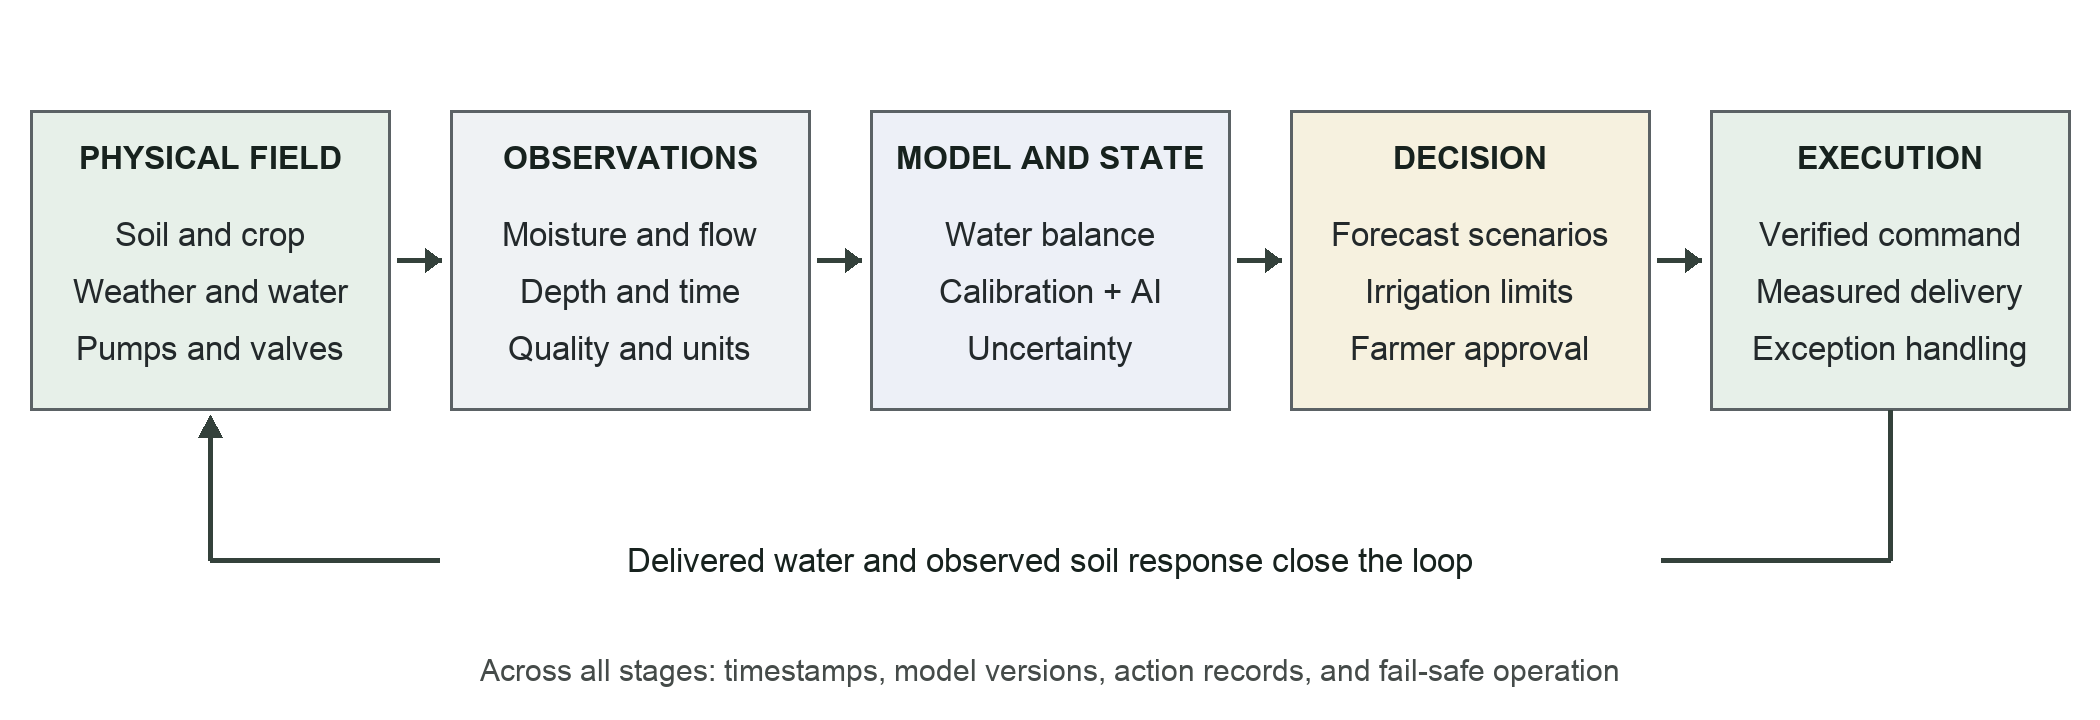
\includegraphics[width=\linewidth]{Figures/irrigation_digital_twin_architecture.png}

\caption{Proposed irrigation-centred digital-twin loop. Measurements of delivered water and subsequent soil response close the loop; a command log alone does not confirm physical execution. This is an original synthesis, not an evaluated deployment.}

\label{fig:architecture}
\Description{Five stages connect the physical field to observations, model and state, decision, and execution. A return path from execution to the field records delivered water and observed soil response. Timestamps, model versions, action records, and fail-safe operation span all stages.}

\end{figure}

Each observation should retain its unit, depth or footprint, timestamp, sensor identity, uncertainty estimate, and quality flag. Surface remote-sensing information and a buried point sensor should not be merged as though they observed the same volume. The model version, parameter set, weather forecast issue time, and accepted action should also be retained. These records make a decision reconstructable and allow errors to be assigned to sensing, modelling, forecasting, or execution.

For the proposed deployment, computationally expensive retraining can occur off-site, while local control retains operational limits and an approved fallback schedule. Stale data, a failed sensor, or unavailable communication should trigger an explicit degraded mode. Such provisions are design requirements advanced here; their cost and reliability must be measured in the deployment rather than assumed from the architecture.


\subsection{A Taxonomy Linking Models to Evidence}
\label{sec:taxonomy}
Figure~\ref{fig:taxonomy} organises the synthesis along four independent axes. The coupling axis adapts the model--shadow--twin distinction \cite{R05}; the remaining axes separate model family, AI role, and evidence level. Unlike a single maturity score, this representation does not imply that increasing neural-network complexity increases operational value. A crop simulator can support a useful decision without being a digital twin, while an automated feedback loop can use a simple calibrated balance.

\begin{figure}[tbp]
\centering
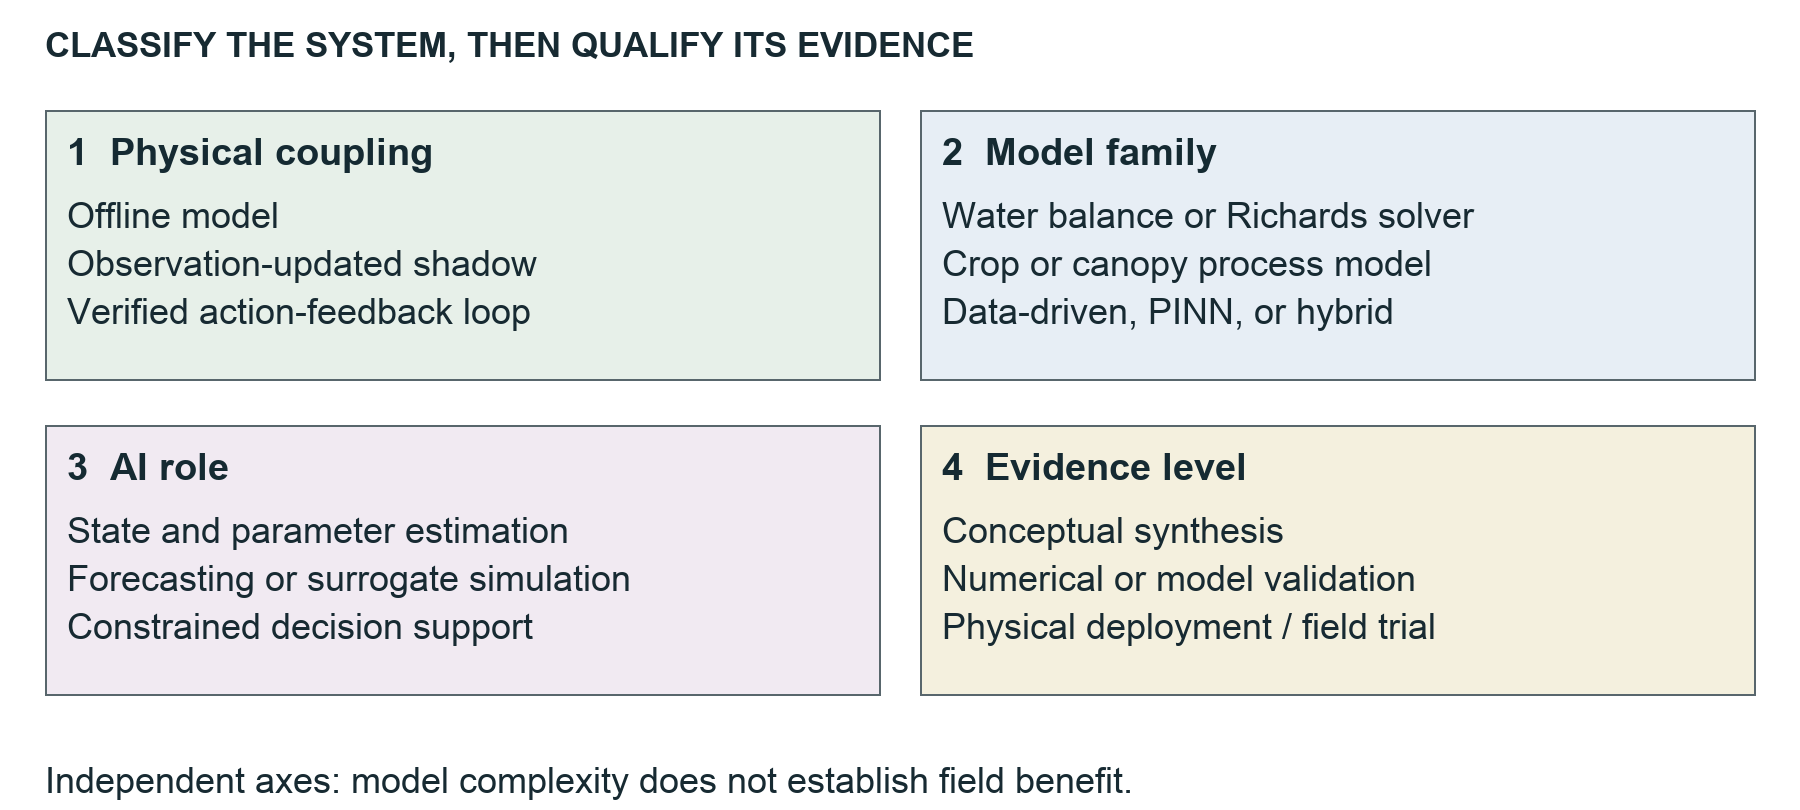
\includegraphics[width=\linewidth]{Figures/taxonomy.png}
\caption{Proposed four-axis taxonomy for interpreting smart-farming digital-twin studies. Categories organise this review; they are not a validated scoring instrument.}
\label{fig:taxonomy}
\Description{Four panels distinguish physical coupling, model family, AI role, and evidence level. Coupling runs from an offline model to observation updates and verified feedback. Evidence ranges from conceptual synthesis through numerical validation to deployment or field trials. The axes are independent.}
\end{figure}

For example, a Richards-based PINN tested with synthetic observations belongs to a different evidence category from a monitored irrigation installation even when both use the term digital twin. A surrogate used inside a controller should be classified by both its approximation role and the control experiment used to assess it. This avoids treating state estimation, offline inverse modelling, and action selection as one undifferentiated AI contribution. Sections~\ref{sec:5-1} and~\ref{sec:5-2} retain the corresponding distinction between parameter calibration and state updating.

\section{Governing Equations and Model Selection}

\label{sec:4}

\subsection{Root-Zone Water Balance}

\label{sec:4-1}

A useful starting point is a root-zone control volume. Over a decision interval with fixed rooting depth, conservation gives:

\begin{equation}
W_{t+1}=W_t+P_t+\eta I_{g,t}+C_t-ET_{a,t}-R_t-D_t.
\label{eq:1}
\end{equation}

Equation~\eqref{eq:1} is the discrete conservation constraint. Here storage W and all interval-integrated fluxes are in millimetres; P is rainfall reaching the soil, $I_{g}$ is gross applied irrigation, $\eta$ is the fraction entering the modelled soil control volume, C is capillary inflow, $ET_{a}$ is actual evapotranspiration, R is runoff, and D is drainage below the root zone. Gross irrigation and the efficiency factor must use the same measurement boundary. Losses already represented by $\eta$ must not be subtracted again as runoff or drainage. A changing root-zone depth requires an additional accounting term or an explicitly moving control volume.

FAO-56 relates crop evapotranspiration and root-zone depletion to irrigation management \cite{R06}. With rooting depth $Z_{r}$ in metres and mean volumetric water content $\bar\theta$, the following quantities make the link explicit:

\begin{equation}
W=1000Z_r\bar\theta,\qquad D_r=1000Z_r(\theta_{FC}-\bar\theta).
\label{eq:2}
\end{equation}

\begin{equation}
TAW=1000Z_r(\theta_{FC}-\theta_{WP}),\qquad RAW=p\,TAW.
\label{eq:3}
\end{equation}

Field capacity and wilting-point water contents are $\theta_{FC}$ and $\theta_{WP}$. TAW is total available water, RAW is readily available water, and p is the allowable depletion fraction. The depletion expression applies to the stated root-zone approximation; saturated or highly layered profiles require more careful treatment. Crop coefficients, stress response, and rooting depth should vary with crop development rather than being treated as universal constants \cite{R06}. A simple balance is transparent and inexpensive, but it cannot resolve wetting fronts or depth-specific sensor responses.

\subsection{Unsaturated Flow and Hydraulic Closure}

\label{sec:4-2}

When the management problem depends on vertical redistribution, infiltration, or layered soils, the one-dimensional Richardson-Richards equation supplies a more detailed description \cite{R07}:

\begin{equation}
\frac{\partial\theta(h)}{\partial t}=\frac{\partial}{\partial z}\left[K(h)\left(\frac{\partial h}{\partial z}+1\right)\right]-S_r(z,t).
\label{eq:4}
\end{equation}

In Equation~\eqref{eq:4}, the vertical coordinate z is positive upward, h is pressure head in metres, time is in days, hydraulic conductivity K is in metres per day, and root extraction $S_{r}$ is in inverse days. This sign convention corresponds to upward-positive water flux q = -K(dh/dz + 1). The formulation assumes a rigid porous medium and liquid-water flow; preferential pathways, hysteresis, and strongly coupled thermal effects are not represented by this equation alone. Surface forcing and a justified lower boundary are required. A free-drainage boundary should not be imposed uncritically where a shallow water table controls flow.

The van Genuchten retention relationship \cite{R08}, combined with the Mualem conductivity model \cite{R09}, provides a common hydraulic closure:

\begin{equation}
S_e=\frac{\theta-\theta_r}{\theta_s-\theta_r}=\left[1+(\alpha|h|)^n\right]^{-m},\qquad m=1-\frac{1}{n},\quad h<0.
\label{eq:5}
\end{equation}

\begin{equation}
K(h)=K_{\mathrm{sat}}S_e^{\ell}\left[1-\left(1-S_e^{1/m}\right)^m\right]^2.
\label{eq:6}
\end{equation}

Equations~\eqref{eq:5} and~\eqref{eq:6} supply the retention and conductivity closures. Residual and saturated water contents are $\theta_{r}$ and $\theta_{s}$; $\alpha$ has units of inverse metres; n exceeds one; $\ell$ is a pore-connectivity parameter; and $K_{sat}$ is saturated hydraulic conductivity. Saturated conditions require the saturated branch, with effective saturation equal to one. These relationships reduce the number of unknown functions, but the parameters still require credible estimation. A smooth retention curve fitted to a limited moisture range can conceal poor behaviour outside that range.

The choice between a bucket balance and a Richards solver should depend on whether additional spatial detail changes the management decision. A complex solver with poorly known boundaries may be less useful operationally than a well-calibrated simpler model. Conversely, averaging a strongly stratified profile can obscure drainage and root stress even when mean moisture appears correct. This trade-off should be tested against independent depth-resolved observations and irrigation outcomes.

\subsection{Crop Coupling and Appropriate Fidelity}

\label{sec:4-3}

Soil water is an intermediate variable, not the final agronomic objective. Crop development determines root exploration and demand, while water stress can alter growth and production. APSIM provides a modular agricultural systems simulation framework \cite{R10}, and AquaCrop explicitly models crop production responses to water \cite{R11}. Neither becomes a digital twin merely by being run on a computer; operational linkage additionally requires observation updates and a traceable decision pathway.

For irrigation, the minimum useful coupling may be a crop-stage-dependent root depth and evapotranspiration demand. A production-oriented study may need biomass and yield responses as well. In greenhouse applications, the relevant model may instead couple canopy structure, radiation, temperature, and water demand. Adding these processes expands parameter uncertainty and validation requirements. The proposed principle is to retain each model component only when its contribution can be assessed against an observable or a decision-relevant error.

\section{Calibration and Data Assimilation}

\label{sec:5}

\subsection{Estimating Parameters Without Confounding Errors}

\label{sec:5-1}

Model calibration estimates model parameters, data assimilation updates the estimated system state as observations become available, and sensor calibration addresses measurement accuracy. These three activities should be documented separately; otherwise, an apparently successful hydraulic calibration may compensate for sensor bias, incorrect irrigation inputs, or unmodelled water-table influence.

Let $\beta$ denote physical parameters and $y_{i}$ an observation with uncertainty scale $\sigma_{i}$. A regularised calibration objective can be written as:

\begin{equation}
\hat{\boldsymbol\beta}=\arg\min_{\boldsymbol\beta\in\mathcal B}\left\{\sum_i\left[\frac{y_i-H_i(x_i(\boldsymbol\beta))}{\sigma_i}\right]^2+\lambda_\beta\left\|L(\boldsymbol\beta-\boldsymbol\beta_0)\right\|_2^2\right\}.
\label{eq:7}
\end{equation}

In Equation~\eqref{eq:7}, the observation operator $H_{i}$ maps model states to the measurement depth or footprint, B imposes admissible parameter bounds, and $\beta_{0}$ encodes prior information. L scales or couples the regularisation terms. This is a proposed generic objective, not a uniquely preferred estimator. With correlated residuals, a covariance-weighted formulation should replace independent squared errors. Model discrepancy and measurement uncertainty should not be assumed interchangeable.

Practical calibration should begin with measured soil texture, bulk density where relevant, sensor response, irrigation flow, and boundary information. A sensitivity analysis can identify which parameters the available observations constrain. Wetting and drying episodes should both be represented. Multiple depths and independently measured irrigation help distinguish storage changes from hydraulic transport; they do not guarantee that every parameter is identifiable. Parameter ensembles or profile-based analyses should be used to expose alternative parameter sets with similar fit.

Randomly splitting adjacent timestamps is particularly weak evidence of generalisation because neighbouring observations share weather, crop stage, and antecedent conditions. A stronger protocol holds out complete events, later periods, another season, or another field. Calibration choices and stopping rules should be fixed before inspecting the final test set. Depth-specific bias and wetting-front timing should be examined alongside aggregate error.

\subsection{Updating States During Operation}

\label{sec:5-2}

The ensemble Kalman filter provides one established approach to sequential estimation \cite{R12}. For a linear observation operator, the familiar analysis update is:

\begin{equation}
\mathbf x^{a}=\mathbf x^{f}+\mathbf G(\mathbf y-\mathbf H\mathbf x^{f}),\qquad \mathbf G=\mathbf P^{f}\mathbf H^{T}\left(\mathbf H\mathbf P^{f}\mathbf H^{T}+\mathbf R\right)^{-1}.
\label{eq:8}
\end{equation}

Equation~\eqref{eq:8} defines the analysis correction. The forecast state $x^{f}$ is corrected using the observation innovation, forecast covariance $P^{f}$, and observation-error covariance R; G is the gain. In an ensemble implementation, covariance is estimated from an ensemble, with further choices needed for nonlinear operators and sampling error. This equation illustrates state updating, not an assurance that all soil-water distributions are Gaussian.

The proposed operational workflow assimilates quality-controlled observations, forecasts several weather scenarios, and records the uncertainty of root-zone depletion. It also logs analysis increments: a state correction can introduce or remove apparent water without a corresponding physical flux. Such increments must be separated from physical water-balance closure. Frequent large corrections are a diagnostic signal to revisit parameters, boundary conditions, sensor bias, or model structure rather than evidence that the underlying model is adequate.

\section{Physics-Informed Learning}

\label{sec:6}

\subsection{Embedding Physical Constraints}

\label{sec:6-1}

Physics-informed neural networks (PINNs) combine observations with differential-equation residuals during training \cite{R13}. The wider physics-informed machine-learning framework also includes architectural constraints and hybrid modelling \cite{R14}. For a network estimating pressure head, the Richards residual can be defined as:

\begin{equation}
r_f(z,t)=\partial_t\theta(\hat h)-\partial_z\left[K(\hat h)(\partial_z\hat h+1)\right]+S_r.
\label{eq:9}
\end{equation}

Equation~\eqref{eq:9} moves all terms of Equation~\eqref{eq:4} to a residual. A suitable training objective distinguishes data, governing physics, initial conditions, boundary conditions, and parameter regularisation:

\begin{equation}
\mathcal L=\lambda_d\mathcal L_d+\lambda_f\mathcal L_f+\lambda_{ic}\mathcal L_{ic}+\lambda_{bc}\mathcal L_{bc}+\lambda_p\mathcal L_p.
\label{eq:10}
\end{equation}

In Equation~\eqref{eq:10}, data loss compares predicted observables with measurements; physics loss evaluates the residual at collocation points. The remaining terms constrain initial and boundary behaviour and admissible parameters. Automatic differentiation supplies the derivatives. Terms should be nondimensionalised or scaled before their weights are chosen, because a numerical balance among incompatible units has no physical interpretation. Joint estimation of network weights and hydraulic parameters is possible, but adding a physical residual does not create information that the measurements cannot identify.

Bandai and Ghezzehei \cite{R15} investigate inverse estimation of constitutive relationships and soil-water flux from moisture measurements using monotonicity constraints. Their subsequent work \cite{R16} evaluates forward and inverse Richards modelling, including domain decomposition for soils with discontinuous hydraulic conductivity. Its comparisons with analytical and conventional numerical solutions establish modelling evidence, not a field-tested claim of irrigation savings. The reported sensitivity to initialisation and computational cost is important when considering online use.

\subsection{Failure Modes and Hybrid Alternatives}

\label{sec:6-2}

PINNs should not be assumed to outperform established numerical solvers. Krishnapriyan et al. \cite{R17} demonstrate optimisation difficulties for representative differential equations as problem complexity increases. A small training loss also does not guarantee accurate extrapolation or exact integral conservation. In a layered soil, physical continuity conditions for pressure and flux require explicit attention; one smooth network can be an unsuitable representation of discontinuous material properties.

For agricultural deployment, the proposed comparison should include a calibrated conventional solver, a purely data-driven predictor, and a hybrid alternative. A PINN may be useful for inverse estimation, while a conservative simulator remains responsible for water accounting. Alternatively, a trained surrogate can accelerate repeated predictions inside a controller. Offline training time, online inference time, retraining frequency, and error under unfamiliar weather should be reported separately. These costs determine whether computational acceleration is real for the complete workflow.

The strongest candidate is therefore not necessarily an end-to-end PINN. A hybrid may use physical storage dynamics, learned forecast corrections, and bounded residual terms. Any learned correction should be checked for long-term drift and changes in mass balance. Physics supplies a useful constraint, but it can also encode an incomplete model of the field. Detecting that incompleteness remains a necessary part of model validation.

\section{Applications and the Strength of Current Evidence}

\label{sec:7}

Table~\ref{tab:1} separates representative contributions by their evidence and unresolved implications. It is a purposive comparison, not a ranking or a complete catalogue. Across these studies, the distinction between a model that predicts, a platform that integrates, and a system that improves management is central.

\begin{table}[!htbp]
\caption{Representative literature and the limits of inference. Review articles supply context; numerical studies and physical deployments answer different validation questions.}
\label{tab:1}
\centering
\small
\begin{tabular}{>{\raggedright\arraybackslash}p{\dimexpr 0.2\linewidth-1.60\tabcolsep\relax}>{\raggedright\arraybackslash}p{\dimexpr 0.23\linewidth-1.84\tabcolsep\relax}>{\raggedright\arraybackslash}p{\dimexpr 0.28\linewidth-2.24\tabcolsep\relax}>{\raggedright\arraybackslash}p{\dimexpr 0.29\linewidth-2.32\tabcolsep\relax}}
\toprule
\textbf{Study focus} & \textbf{Evidence level} & \textbf{Contribution} & \textbf{Limit of inference} \\
\midrule
Architecture and adoption \cite{R01,R02,R03} & Conceptual synthesis and reviews & Management loops and integration pathways & Not a controlled estimate of water savings \\
Interoperability \cite{R04} & Systematic review by the cited authors & Semantics and cross-asset integration gaps & A review-level finding, not a deployment test \\
Soil-water PINNs \cite{R15,R16} & Inverse modelling and numerical validation & Hydraulic inference and layered-soil modelling & Does not demonstrate seasonal farm benefits \\
Irrigation control \cite{R18} & Numerical control study; preprint & Surrogate prediction and zone control & Requires independent field validation \\
Water-salt management \cite{R19} & Reported physical irrigation-drainage deployment & Monitoring, forecasting, and operational integration & Site-specific and multi-component evidence \\
Greenhouse management \cite{R20} & Greenhouse case study & Canopy and environmental model integration & Transfer to open fields is not established \\
\bottomrule
\end{tabular}

\end{table}

Precision irrigation is the most direct application of the technical framework developed here. Huang et al. \cite{R18} describe a neural-network approximation used in zone model predictive control to keep root-zone soil moisture within a target region while reducing irrigation. Their preprint supports the relevance of computationally tractable prediction and control; its numerical results should not be presented as established field performance.

Qin et al. \cite{R19} report a digital-twin-enabled irrigation-drainage system for saline agroecosystems that combines environmental monitoring, forecasting, and automated control. The reported setting demonstrates why moisture alone may be insufficient: irrigation decisions can also affect salt redistribution and groundwater interactions. This review does not extract a universal water-saving percentage from that platform. Transfer to another crop or soil requires a new assessment, and improvements in a multi-component system cannot automatically be attributed to the digital twin or AI model in isolation.

Greenhouse management extends the same reasoning to energy and microclimate. Xu et al. \cite{R20} describe a digital-twin approach using functional-structural plant modelling in a Beijing solar greenhouse case study. That modelling perspective links canopy representation with environmental management, but conclusions from a bounded greenhouse setting should not be transferred directly to open fields. Temperature, light, and water decisions can interact, so an irrigation-only objective may overlook energy or crop-quality consequences.

At the broader smart-farming level, the reviews cover crop monitoring, livestock, machinery, and other management contexts \cite{R02,R03}. The equations in this paper are not a universal model for those applications. What transfers is the evaluation logic: define the physical entity, specify the observation and feedback pathways, validate the model at the relevant scale, and measure the consequence of the decision. Extending the irrigation framework to livestock or machinery would require different governing models and domain-specific outcomes.


\subsection{Study-Level Comparison of Methods and Data}
\label{sec:study-comparison}
Table~\ref{tab:study-methods} specifies the data and methodology behind four representative applications, while Table~\ref{tab:study-findings} separates their findings from this review's interpretation. The two tables share study identifiers to keep their text readable at the ACM column width. The selection spans numerical hydrology, simulated irrigation control, a water--salt platform, and a greenhouse case; it is not an exhaustive benchmark.

\begin{table}[tbp]
\caption{Methods and data in selected studies. A named public dataset is not assumed when it could not be verified from the consulted source.}
\label{tab:study-methods}
\centering
\begin{tabularx}{\linewidth}{@{}>{\raggedright\arraybackslash}p{0.19\linewidth}YY@{}}
\toprule
Study & Approach and methodology & Data or evaluation setting \\
\midrule
Bandai and Ghezzehei \cite{R16} & Richards PINNs with domain decomposition; forward and inverse tests & Analytical and numerical comparisons; noisy HYDRUS-1D-generated moisture; code and data archive linked by authors \\
Huang et al. \cite{R18} & Two-layer neural surrogate, bias correction, and zone model predictive control & Simulated one-dimensional soil profile with grass and sandy loam; open- and closed-loop tests against an LSTM baseline \\
Qin et al. \cite{R19} & IoT sensing, LSTM forecasting, and integrated irrigation--drainage management & Saline agricultural plots in northwestern China; moisture, temperature, and salinity monitoring; reusable dataset identifier not verified \\
Xu et al. \cite{R20} & Digital twin with functional--structural plant modelling & Solar greenhouse case in Beijing; canopy and environmental representation; public dataset identifier not verified from publisher summary \\
\bottomrule
\end{tabularx}
\end{table}

\begin{table}[tbp]
\caption{Reported contributions and critical limits of the studies in Table~\ref{tab:study-methods}. Limits are this review's interpretation, not additional experimental findings.}
\label{tab:study-findings}
\centering
\begin{tabularx}{\linewidth}{@{}>{\raggedright\arraybackslash}p{0.19\linewidth}YY@{}}
\toprule
Study & Finding supported by consulted source & Limit for smart-farming decisions \\
\midrule
Bandai and Ghezzehei \cite{R16} & Layered-soil solutions and inverse surface-flux estimation; sensitivity to training configuration & Numerical evidence, not seasonal irrigation benefit; hydraulic properties known in the cited inverse test \\
Huang et al. \cite{R18} & Improved surrogate prediction against its LSTM comparator and computationally tractable zone control & Simulation and preprint evidence; no measured farm-scale water or yield effect established here \\
Qin et al. \cite{R19} & Reported field water--salt management and salinity-control benefits in an integrated system & Multiple interventions; separate AI contribution and transferability need controlled assessment \\
Xu et al. \cite{R20} & Canopy-light representation supporting greenhouse design and management & Publisher-summary access limits extraction; no general open-field irrigation saving can be inferred \\
\bottomrule
\end{tabularx}
\end{table}

The comparison reveals different validation targets. Bandai and Ghezzehei \cite{R16} test a numerical inverse problem; their linked code and data support reproducibility of that task, not a claim of farm deployment. Huang et al. \cite{R18} move from prediction to simulated control, but the surrogate and controller are evaluated within specified model assumptions. Qin et al. \cite{R19} provide a physical management setting, while the combined sensing, water reuse, drainage, and forecasting components complicate attribution. Xu et al. \cite{R20} show why crop geometry and greenhouse environment require a different modelling boundary. Thus, numerical accuracy, integration feasibility, and agronomic effectiveness are separate conclusions rather than successive synonyms for success.

For this review, the appropriate comparison unit is therefore a complete decision episode: observed state, forecast issue time, model version, feasible action set, selected action, measured delivery, and subsequent soil or crop response. This is a proposed reporting unit, not one claimed to be available in every cited dataset. It would expose whether an apparent improvement comes from better sensing, better state estimation, a different objective, or a genuinely better decision under the same information.

\section{From Model Predictions to Measurable Decisions}

\label{sec:8}

\subsection{Constrained Irrigation Optimisation}

\label{sec:8-1}

The following model predictive control formulation is proposed as an organising example, informed by the control setting in \cite{R18}. At each decision time, estimate the current state, forecast over H intervals, optimise an irrigation sequence, execute only its first action, and repeat after new observations. A dimensionally normalised objective is:

\begin{equation}
\min_{u_{0:H-1}}\sum_{k=1}^{H}\left[a\left(\frac{u_{k-1}}{U_0}\right)^2+b\left(\frac{s_k}{S_0}\right)^2+c\left(\frac{d_k}{D_0}\right)^2\right].
\label{eq:11}
\end{equation}

In Equation~\eqref{eq:11}, u is gross irrigation depth, s is depletion above the chosen stress threshold, and d is deep drainage; $U_{0}$, $S_{0}$, and $D_{0}$ are positive reference depths. The weights a, b, and c express management priorities rather than universal constants. Constraints include available water, pump capacity, permissible operating windows, soil infiltration limits, and maximum allowable crop stress. Saline soils may require planned leaching, so penalising all drainage would be inappropriate. A crop- and site-specific formulation must distinguish beneficial leaching from avoidable losses.

Weather ensembles and parameter ensembles can reveal whether a recommendation is sensitive to uncertainty. The proposed controller should report that sensitivity and defer to a predefined fallback when its operating conditions are not met. Choosing among uncertain actions requires an explicit risk preference; widening an uncertainty interval without changing the decision rule is not, by itself, risk-aware management.

\subsection{Illustrative Calculation}

\label{sec:8-2}

Consider an assumed one-hectare field with a uniform 0.40 m root zone, field-capacity water content of 0.30, wilting-point water content of 0.15, and allowable depletion fraction of 0.50. Equations~\eqref{eq:2} and~\eqref{eq:3} give total available water of 60 mm and readily available water of 30 mm. A mean water content of 0.24 corresponds to depletion of 24 mm.

If the next interval removes 6 mm by evapotranspiration, with no rainfall, capillary rise, runoff, or drainage, depletion reaches 30 mm. Suppose irrigation is then applied to reduce depletion to a chosen target of 12 mm. The required net addition is 18 mm. With an assumed 0.90 fraction of gross irrigation entering the control volume, gross application is 20 mm. The volume conversion is:

\begin{equation}
I_g=\frac{30-12}{0.90}=20\ \mathrm{mm},\qquad V=\frac{I_g}{1000}A=200\ \mathrm{m^3},\quad A=10{,}000\ \mathrm{m^2}.
\label{eq:12}
\end{equation}

Equation~\eqref{eq:12} converts the assumed depletion deficit to an applied volume. These are illustrative assumptions, not observed crop parameters or an optimised recommendation. The 12 mm target is selected solely to demonstrate the calculation. Actual timing must respect infiltration, equipment capacity, weather forecasts, and the interval during which crop stress might develop. An uncertainty of 0.02 in mean volumetric water content corresponds to 8 mm of root-zone storage in this example. That sensitivity shows why a precise-looking recommendation can be poorly supported even when average predictive performance appears acceptable.

\subsection{Metrics and an Evaluation Protocol}

\label{sec:8-3}

Table~\ref{tab:2} proposes outcome definitions that keep modelling performance distinct from management benefit. In particular, irrigation withdrawal or application is not identical to consumptive water use. Reduced pumping can coexist with unchanged evapotranspiration, and altered drainage can affect downstream availability. A study must identify the water-accounting boundary before claiming savings.

\begin{table}[!htbp]
\caption{Proposed minimum reporting set. Metrics should be accompanied by uncertainty, the measurement boundary, and the relevant comparison period.}
\label{tab:2}
\centering
\small
\begin{tabular}{>{\raggedright\arraybackslash}p{\dimexpr 0.2\linewidth-1.20\tabcolsep\relax}>{\raggedright\arraybackslash}p{\dimexpr 0.4\linewidth-2.40\tabcolsep\relax}>{\raggedright\arraybackslash}p{\dimexpr 0.4\linewidth-2.40\tabcolsep\relax}}
\toprule
\textbf{Outcome} & \textbf{Metric or unit} & \textbf{Interpretation requirement} \\
\midrule
Moisture prediction & RMSE and bias in volumetric water content, by depth and horizon & Independent observations and event-level holdouts \\
State uncertainty & Interval coverage and width; threshold exceedance reliability & Coverage alone can reward uninformative intervals \\
Water accounting & Storage change minus net physical inflow, in mm & Report assimilation increments separately \\
Irrigation delivery & Metered gross depth (mm) and volume (m\ensuremath{^3}) & Define field area, meter location, and evaluation period \\
Consumptive use & Actual evapotranspiration (mm), measured or independently estimated & Do not equate it with water pumped or applied \\
Agronomic response & Marketable yield (kg/ha), quality, and stress exposure & Use an appropriate replicated comparator \\
Water productivity & Yield / applied irrigation, or yield / actual ET (kg/m\ensuremath{^3}) & State the denominator; these are different measures \\
Operational value & Missed actions, uptime, costs, and operator effort & Include installation, maintenance, and failure recovery \\
\bottomrule
\end{tabular}

\end{table}

The proposed validation sequence begins with retrospective testing on held-out events or seasons. It proceeds to prospective shadow operation, where recommendations are recorded but not executed, and then to supervised field trials. Comparators should include the current farm schedule and a credible simple baseline, such as a calibrated depletion-threshold controller. Ablations should separate the effects of new sensors, assimilation, learned components, and optimisation.

Where feasible, field trials should allocate treatments across independent plots or irrigation zones with replication, account for spatial variation, and cover more than one season. Statistical independence belongs to the experimental unit, not to each sensor timestamp. Report seasonal applied volume, marketable yield or quality, stress exposure, failure events, maintenance effort, and uncertainty in treatment differences. Yield non-inferiority margins and primary outcomes should be specified before examining results. No trial or power calculation is claimed in this review; these are requirements for subsequent empirical work.


Figure~\ref{fig:evaluation} makes the evaluation sequence explicit. Moving from retrospective fit to shadow operation is conditional on data-quality, uncertainty, and conservation checks; moving to actuation additionally requires operational safeguards. The stages do not certify safety by themselves. They identify which evidence must exist before the next claim can be investigated, using the outcome definitions in Table~\ref{tab:2} and the illustrative sensitivity in Section~\ref{sec:8-2}.

\begin{figure}[tbp]
\centering
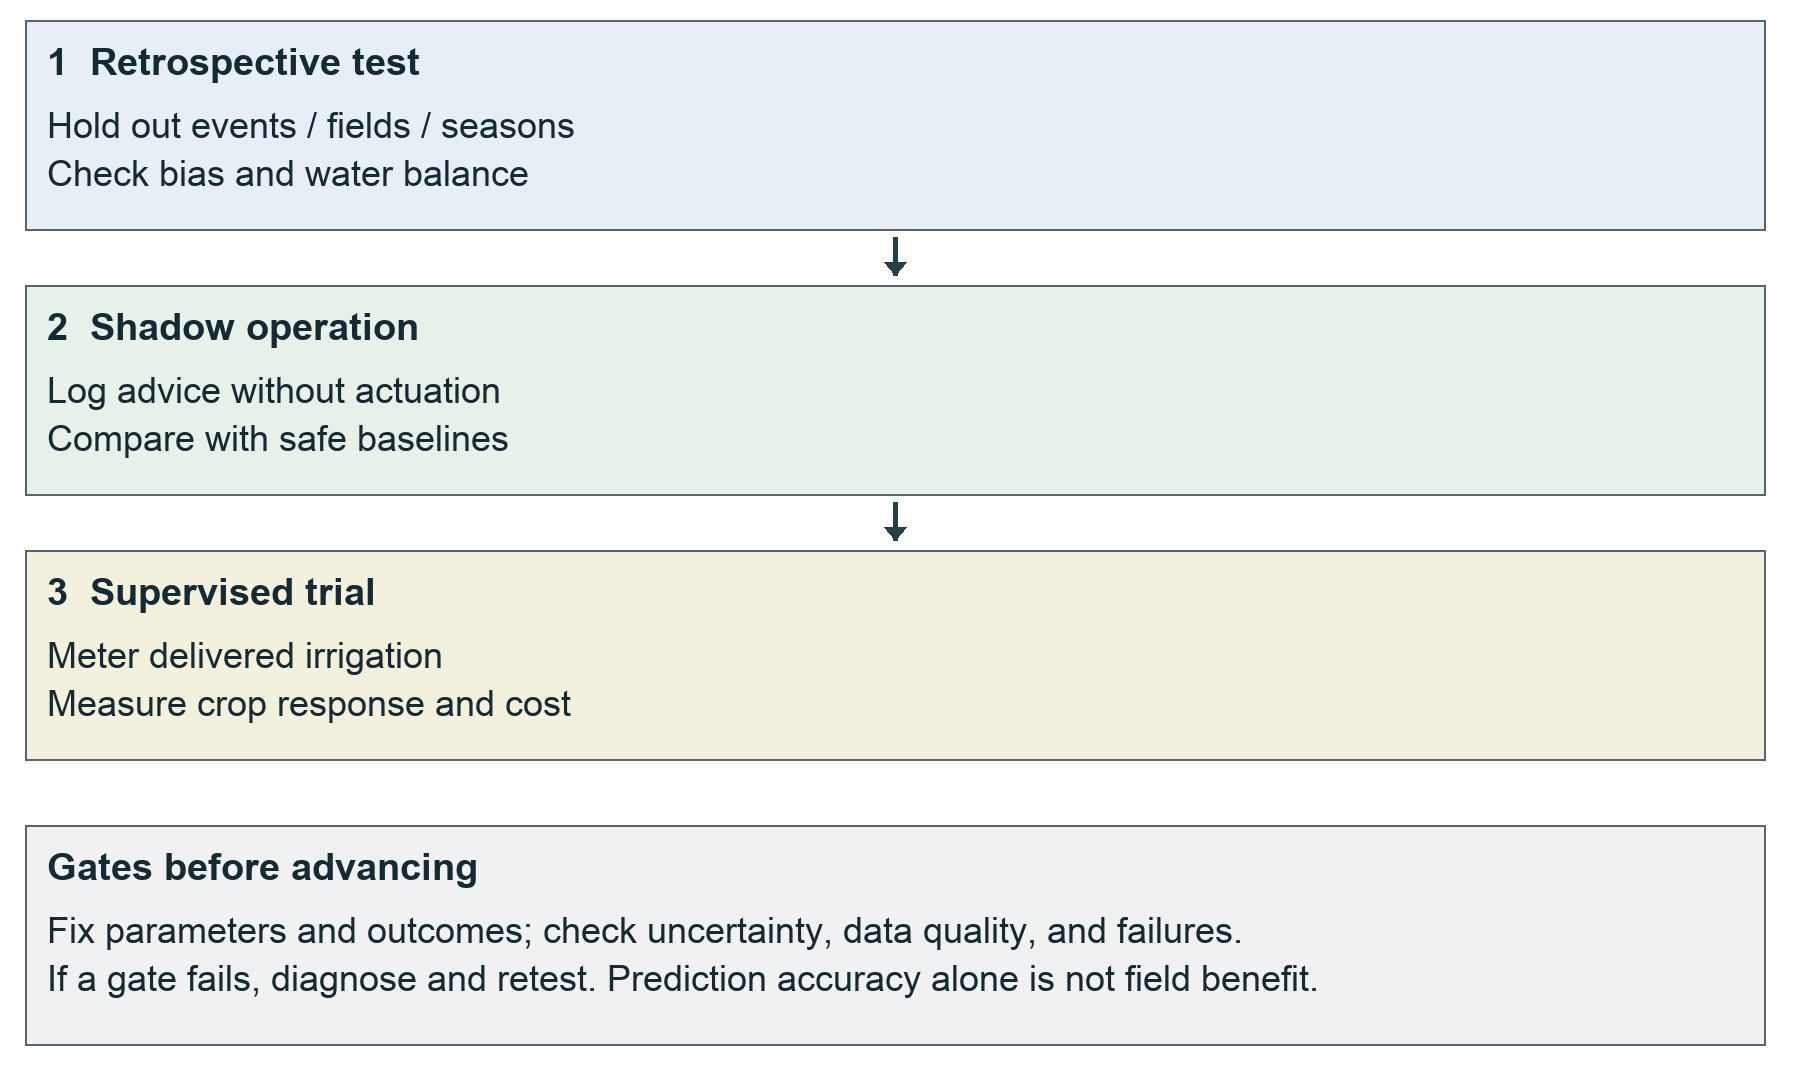
\includegraphics[width=\linewidth]{Figures/evaluation_flow.png}
\caption{Proposed staged evaluation workflow. Advancement depends on documented checks, not merely on completion of model training.}
\label{fig:evaluation}
\Description{A top-to-bottom flow progresses from retrospective holdout testing to non-actuating shadow operation and then supervised field trials. A shared gate requires fixed parameters and outcomes, uncertainty reporting, data-quality checks, and failure analysis. Failed gates return the system to diagnosis and testing.}
\end{figure}

\section{Research Directions and Deployment Constraints}

\label{sec:9}

Decision-aware calibration is a priority. Minimising average moisture error can give too little weight to mistakes near an irrigation threshold. Future studies should evaluate whether parameters calibrated to event timing, depletion exceedance, or action regret improve decisions while retaining physical plausibility. The comparison must be made on held-out events rather than by selecting a favourable objective retrospectively.

Identifiability-aware sensing is equally important. Additional sensors should be evaluated for the uncertainty or decision ambiguity they remove. A flow meter, water-table observation, or extra measurement depth may be more informative than another surface probe. Active sensing and experimental irrigation pulses are promising research designs, but they require agronomic safeguards and a quantified value-of-information analysis.

Hybrid models need better conservation and uncertainty tests. A useful benchmark would contain known irrigation inputs, multiple soil depths, hydraulic measurements, weather, and crop observations, with entire fields and seasons reserved for testing. It should assess water-balance residuals, interval calibration, inference cost, and decision outcomes together. This proposed benchmark would allow a PINN, a numerical solver, and a simpler balance model to be compared under the same information constraints.

Interoperability must include meaning, not only message transport. The fragmentation identified in \cite{R04} motivates portable descriptions of observation depth, management zones, crop stage, model parameters, and executed actions. Versioned data and model records should make it possible to reconstruct why a recommendation changed. A vendor-independent export of measurements and decisions is also important for continuity when equipment or software providers change.

Deployment research must address affordability and failure recovery. The relevant cost includes installation, replacement sensors, calibration visits, communications, computation, and operator time. A farmer should be able to understand the proposed action, override it, and see whether delivery matched the plan. Access control and authenticated commands are particularly important when the model can actuate pumps or valves. These are proposed operational requirements, not evidence that any reviewed platform already satisfies them.

Finally, transferability should be tested deliberately. A model validated in one soil, crop, or greenhouse may fail under another rooting pattern, salinity regime, irrigation method, or connectivity condition. Multi-season and multi-site evaluations should therefore distinguish parameters that transfer, parameters needing recalibration, and processes that require a different model. A defensible system should be able to decline an unsupported recommendation rather than conceal unfamiliar conditions behind a confident forecast.


\subsection{Research Gaps as Falsifiable Comparisons}
\label{sec:gaps}
The preceding directions become useful research questions only when the proposed improvement can fail a stated test. Table~\ref{tab:gaps} links four gaps to comparisons and measurable outcomes. These experiments are proposed work; the present review supplies neither datasets nor effect estimates for them.

\begin{table}[tbp]
\caption{Evidence-linked research agenda. Outcomes and decision thresholds should be specified before inspecting test results.}
\label{tab:gaps}
\centering
\begin{tabularx}{\linewidth}{@{}>{\raggedright\arraybackslash}p{0.25\linewidth}YY@{}}
\toprule
Gap and motivation & Proposed comparison & Observable outcome \\
\midrule
Fit versus action quality \cite{R16,R18} & Moisture-error calibration versus decision-aware calibration with identical sensors and control constraints & Held-out threshold violations, metered irrigation, and crop-stress exposure \\
Learned model versus physical accounting \cite{R14,R16,R17} & PINN or hybrid versus calibrated balance and numerical solver under matched inputs & Moisture bias, water-balance residual, interval reliability, and runtime \\
Platform benefit versus component contribution \cite{R19} & Replicated trials separating sensor, forecast, and control changes & Applied volume, salinity, yield, failures, and maintenance cost \\
Site fit versus transportability \cite{R04,R20} & Frozen model versus local recalibration across fields or seasons & Performance loss, recalibration effort, fallback frequency, and decision stability \\
\bottomrule
\end{tabularx}
\end{table}

A negative result would also be informative. If a complex hybrid fails to improve decisions over a calibrated threshold rule despite reducing average moisture error, the extra modelling detail may not justify its cost for that deployment. If benefits disappear when the same sensors are supplied to the baseline, the contribution is sensing rather than the AI architecture. If a model needs frequent re-estimation at each site, claims of transfer should be replaced with an explicit account of recalibration cost. These interpretations follow from the comparison design, not from an assumption that one class of model must win.

\subsection{Data Governance and Operational Responsibility}
\label{sec:governance}
The proposed decision record can reveal farm schedules, resource constraints, and commercially sensitive production information. A deployment should specify who may access observations, change parameters, approve actions, and retain exported records. Farmers need an intelligible reason for a recommendation and a usable override. An explanation does not prove the recommendation is correct: measured delivery, agronomic constraints, and failure recovery remain necessary. These are design implications of the proposed architecture, not claims that the reviewed systems have been audited against a common governance standard.

\section{Conclusion}

\label{sec:10}

The convergence of AI and digital twins can support smart farming when observations, models, and decisions are connected through a verifiable physical loop. For precision irrigation, governing equations make storage and flux assumptions explicit; calibration links model parameters to local evidence; assimilation updates the estimated state; and physics-informed learning offers additional tools for constrained approximation and inverse modelling. None of these components independently establishes practical benefit.

The review argues for evaluating the full chain from soil-moisture estimation to irrigation execution and crop response. A convincing system must account for uncertainty, identify its limits of validity, and compare measured water and production outcomes against credible alternatives. PINNs deserve investigation within that chain, but not exemption from comparison with simpler models or conventional solvers. The proposed architecture and worked example provide a technical basis for subsequent research, while controlled field validation remains necessary before any claim of improved water consumption, yield, or economic return.


The three review questions therefore have distinct answers. Operational linkage requires an observed and auditable feedback path, not simply a detailed visual replica. Physical equations and calibrated parameters establish interpretable constraints, while assimilation and physics-informed learning address different estimation tasks. Practical value requires independent measurement of delivered water, soil response, and crop outcomes against credible comparators. The immediate research priority is to test that full chain under matched information and held-out conditions, using the comparisons in Section~\ref{sec:gaps}. This conclusion is bounded by the purposive corpus and heterogeneous evidence described in Section~\ref{sec:extraction}.

\section{Research Transparency}

\label{sec:transparency}

This manuscript is an AI-assisted review draft prepared for researcher review. It reports no new experiment, dataset, or measured treatment effect. The architecture, control formulation, and evaluation protocol are proposed synthesis; the numerical irrigation example is illustrative. The cited control preprint is identified separately from peer-reviewed sources. Generative AI tools assisted drafting and revision. Codex assisted the ACM conversion, literature-source checks, original diagram preparation, and cross-reference verification; the earlier Prism-approved calibration paragraph is retained. Responsibility for the final scientific interpretation and attribution remains with the author. Bibliographic existence and compilation checks do not constitute independent validation of each scientific claim.

\bibliographystyle{ACM-Reference-Format}

\bibliography{references}

\end{document}
